\documentclass[12pt]{article}
\usepackage[utf8]{inputenc}
\usepackage{geometry}
\usepackage{graphicx}
\usepackage{amsmath}

\geometry{a4paper}

\title{Technical Report - FarmClash}
\author{Camille De Vuyst, Joren Van der Sande, Thomas De Volder,\\ Faisal Ettarrahi, Ferhat Van Herck, Siebe Mees}
\date{\today}

\begin{document}

\maketitle
\tableofcontents
\newpage

\begin{abstract}
This technical report describes the development and implementation of FarmClash, a web-based idle game designed for the Programming Project Databases course at the University of Antwerp. The game integrates concepts of resource management and multiplayer interaction within a farm management context, drawing inspiration from popular titles like Clash of Clans and Hay Day.
\end{abstract}

\section{Introduction}
FarmClash is an educational project designed to apply database and web development skills in a practical scenario. Inspired by games like Clash of Clans and Hay Day, it challenges players to manage a farm, interact with other players, and strategize in real-time, balancing competitive and cooperative gameplay elements.

\section{Project Objectives}
The primary objectives of this project include:
\begin{itemize}
    \item Develop a functional web-based idle game, inspired by titles such as Grepolis and Clash of Clans, focusing on the management of cities and resources.
    \item Utilize PostgreSQL to manage a robust database that handles game states, user data, and interactive features such as guilds and direct messaging.
    \item Implement secure and efficient server-side interactions using Flask, ensuring that the system handles real-time data exchange and multiplayer interactions seamlessly.
    \item Create an intuitive user interface that facilitates easy navigation and management of game tasks, utilizing technologies such as React for dynamic frontend development and CSS frameworks for aesthetic design.
    \item Design the game to support background updates and cooldowns effectively, representing idle game mechanics where actions continue to progress even when players are not actively engaged.
    \item Implement software extensibility and maintainability, preparing the system for future upgrades and scalability.
    \item Deploy and maintain the software system on a production environment, leveraging provided Google Cloud Platform resources for hosting.
\end{itemize}
This project is designed to meet the educational goals of learning to develop extensive software projects within a team setting, discovering and integrating new technologies, and effectively planning and distributing tasks.


\section{Game Description}
FarmClash allows players to build and manage their farms, defend against attacks from other players, and maximize their profits through strategic selling of farm produce influenced by dynamic market prices. Players start with a basic farm and can upgrade their facilities and defenses as they progress, interacting with other players through alliances and competitive gameplay.
\subsection{Buildings}

\subsubsection{Idle Buildings}

\begin{enumerate}
    \item \textbf{Chickencoop}: Produces eggs and allows breeding of chickens. Higher levels yield more products and increases the limit of chickens.
    \item \textbf{Cowbarn}: Produces milk and allows breeding of cows. Higher levels yield more products and increases the limit of cows.
    \item \textbf{Goatbarn}: Produces wool and allows breeding of goats. Higher levels yield more products and increases the limit of goats.
    \item \textbf{Pigpen}: Produces truffles and allows breeding of pigs. Higher levels yield more products and increases the limit of pigs.
    \item \textbf{Field}: Used for planting crops. Higher levels yield more harvest. (Passive upgrades increase farm time)
\end{enumerate}

\subsubsection{Defense Buildings}

\begin{enumerate}
    \item \textbf{Fence}:
    Increases defense level. Higher level increases the defense level severely. Fortifying can increment the defense level slightly.
    \item \textbf{Townhall}: Determines user level, prevents buildings from leveling beyond its level, unlocks crops, allows the user to discover more of the map, can be fortified for increased defense and researched for a higher attack level, however upgrading does more to the defense and attack level. This building will open a Townhall UI where Next unlocks can be viewed as well as the defense level and base attack level.
\end{enumerate}

\subsubsection{Storage Buildings}

\begin{enumerate}
    \item \textbf{Silo}: Stores crops. Level 10 removes storage limit. Organizing can increment the limit slightly, however upgrading does more to the limit. This building will open a Silo UI. This building will open a Barn UI where resources can be viewed and removed.
    \item \textbf{Barn}: Stores resources besides crops and money. Level 10 removes storage limit. Organizing can increment the limit slightly, however upgrading does more to the limit. This building will open a Barn UI where resources can be viewed and removed.
\end{enumerate}

\subsubsection{Explore Buildings}

\begin{enumerate}
    \item \textbf{Bunny Bay}: Exploring is unlocked as soon as the building reaches level 1. The higher the level, the lower the risk. Investing in the building will also lower the risk slightly. This building will open an Explore UI.
\end{enumerate}

\subsubsection{Friend-placed Buildings}

\begin{enumerate}
    \item \textbf{Gift Boxes}: Friends can place gift boxes once a day with gifts for you. Gifting to others increases your defense level (depending on what and how much you gift).
\end{enumerate}

\subsection{Exploring}

\subsubsection{Exploration Mechanics}

The bunny of the Bay will embark on an exploration journey for a duration chosen by the user, accompanied by a selection of animals chosen by the user, with the exploration time capped by the building level.

During exploration, the user can open the gathered boxes, ensuring there is enough space in storage buildings. The longer the exploration duration, the higher the risk and the average number of resources per box obtained.

A higher building level results in lower risk, higher average resources per box, and higher standard deviation of resources.

Additionally, a higher augment level of the building reduces the risk.

The number of boxes and surviving animals is predetermined at the start of exploration.

Risk chance is calculated as follows:
A : \text{Augment Level}
L : \text{Building Level}
d : \text{Duration}

\[
R(d) =
\begin{cases}
0 & \text{if } d = 1 \\
5 & \text{if } d = 20 \\
10 & \text{if } d = 60 \\
30 & \text{if } d = 180 \\
50 & \text{if } d = 720 \\
70 & \text{if } d = 1440 \\
\end{cases}

\text{Risk}(d, L, A) =
\begin{cases}
100 & \text{if } L = 0 \\
\max\left(0, \frac{R(d)}{L}\right) & \text{if } L \neq 0 \text{ and } A = 0 \\
\max\left(0, \frac{R(d)}{L} + 1 - \left(\frac{3 \log_6 (A + 1)}{2 (A + 1)}\right)\right) & \text{if } L \neq 0 \text{ and } A \neq 0
\end{cases}
\]

The base amount of rewards X is between 0 and 3. If a random integer between 0 and 100 is larger than X \times Risk, then X boxes will be generated.

A box can contain:

\begin{itemize}
    \item Coin (Base: 25\%)
    \item Crop (Base: 25\%)
    \item Animal product box (Base: 25\%)
    \item Raw material box (Base: 15\%)
    \item Empty box (Base: 10\%)
\end{itemize}

The types of crops are limited to the building level.

The more animals sent to explore, the more boxes will be returned. The chance that an animal survives is 100\%−Risk (with slight variations for chickens).

Every surviving animal brings one box, except for cows, which may bring no boxes, and goats, which may bring up to 3 boxes.

Choosing which animals to send on the exploration has its perks and downsides.


\begin{itemize}
    \item \textbf{Chickens}:
    \begin{itemize}
        \item Increased yield of eggs if found.
        (50\% if animal product box is found.)
        \item Increased amount of crops if found.
        (First surviving chicken \cdot1.35, Second surviving chicken \cdot1.35^2 ...).
        \item Increased spread of amount of crops if found.
        (First surviving chicken \cdot1.15, Second surviving chicken \cdot1.15^2 ...).
        \item Higher rarity of animal resources.
        \item Lower chance of getting home safe
        (First surviving chicken -5\%, Second surviving chicken -10\% ...).
    \end{itemize}
    \item \textbf{Cows}:
    \begin{itemize}
        \item Increased yield of milk if found.
        (50\% if animal product box is found.)
        \item Brings more resources on average.
        (First cow \cdot1.25, Second cow \cdot1.25^2 ...).
        \item Higher chance to bring coins.
        (First surviving cow +5\%, Second surviving cow +10\% ...).
        \item Lower chance to bring a box.
        (First surviving cow -10\%, Second surviving cow -20\% ...).
    \end{itemize}

    \item \textbf{Pigs}:
    \begin{itemize}
        \item Increased chances of truffles.
        (50\% if animal product box is found.)
        \item Higher rarity of craft resources if found.
        \item Higher amount of craft resources if found.
        (First surviving pig \cdot1.35, Second surviving pig \cdot1.35^2 ...).
        \item Higher chance of empty boxes.
        (First surviving pig +15 weight, Second surviving pig +30 weight ...).
    \end{itemize}

\item \textbf{Goats}:
\begin{itemize}
    \item Increased chances of wool.
    (50\% if animal product box is found.)
    \item Has a chance to bring 2 boxes.
    (10\% + (0.5\% for the first surviving goat, 1\% for the second surviving goat ...))
    \item Has a small chance to bring 3 boxes.
    (5\% + (0.5\% for the first surviving goat, 1\% for the second surviving goat ...))
    \item Brings lower resources on average.
    (First pig \cdot0.95, Second pig \cdot0.95^2 ...).
\end{itemize}
\end{itemize}


\subsection{Animals}
- Can be sent on explorations.
\begin{enumerate}
    \item Chicken
    \item Cow
    \item Pig
    \item Goat
\end{enumerate}

\subsection{Attacking}

The attack functionality in this Flask application is designed to manage and execute virtual attacks between users. This functionality includes selecting an opponent, displaying attack animations, and determining the result of an attack. It ensures that only authenticated users can participate in these actions, leveraging user session data and custom logic to facilitate fair and engaging interactions.

\subsubsection{Key Components}

\paragraph{Selecting an Opponent}
When a user decides to attack, the system first identifies a suitable opponent. This is done through a function that:
\begin{itemize}
    \item Excludes the current user and their friends.
    \item Filters out users who have been recently searched.
    \item Considers only users whose defense score is within a certain range of the current user's attack score.
    \item Sorts potential opponents by their scores and selects the most suitable one.
\end{itemize}

\paragraph{Rendering Attack Views}
The system provides different views for the attack process:
\begin{itemize}
    \item \textbf{Visit Opponent's World}: Displays the selected opponent’s virtual world.
    \item \textbf{Attack Animation}: Shows an animation of the attack sequence.
    \item \textbf{Attack Result}: Presents the outcome of the attack, detailing whether the user won or lost and the resources gained or lost.
\end{itemize}

\paragraph{Determining Attack Outcomes}
The outcome of an attack is determined based on the attack and defense scores of the user and their opponent:
\begin{itemize}
    \item If the score difference is significant, the outcome is more predictable (win or lose).
    \item For close scores, the outcome may be decided randomly to add an element of chance.
\end{itemize}
The system calculates the resources to be transferred based on the result:
\begin{itemize}
    \item If the user wins, they gain a percentage of the opponent’s resources.
    \item If the user loses, they lose a similar percentage of their resources to the opponent.
\end{itemize}

\paragraph{Updating Resources}
Following the attack, the system updates the resource counts for both the user and their opponent:
\begin{itemize}
    \item Resources are incremented or decremented based on the attack result.
    \item This ensures that the game’s resource economy reflects the outcomes of user interactions accurately.
\end{itemize}

\paragraph{Summary}
This attack functionality is a crucial part of the application, providing an engaging way for users to interact and compete. It carefully manages the selection of opponents, rendering of attack sequences, determination of outcomes, and updates to resources, ensuring a balanced and dynamic user experience.





\subsection{Resources}

\begin{enumerate}
    \item \textbf{Coins}: Used for various purposes. Like upgrading, fortifying, investing...
    \item \textbf{Crops}: Various crops with increasing unlock levels. Total amount limited by Silo capacity.
    \begin{enumerate}
        \item Wheat (Level 0)
        \item Carrot (Level 1)
        \item Corn (Level 2)
        \item Lettuce (Level 3)
        \item Tomato (Level 4)
        \item Turnip (Level 5)
        \item Zucchini (Level 6)
        \item Parsnips (Level 7)
        \item Cauliflower (Level 8)
        \item Eggplant (Level 9)
    \end{enumerate}
    \item \textbf{From Animals}:
    \begin{enumerate}
        \item Egg (Common)
        \item Rustic Egg (Uncommon)
        \item Crimson Egg (Rare)
        \item Emerald Egg (Epic)
        \item Sapphire Egg (Legendary)
        \item Milk (Common)
        \item Chocolate Milk (Uncommon)
        \item Strawberry Milk (Rare)
        \item Blueberry Milk (Epic)
        \item Soy Milk (Legendary)
        \item Wool (Common)
        \item Alpaca Wool (Uncommon)
        \item Cashmere Wool (Rare)
        \item Dolphin Wool (Epic)
        \item Irish Wool (Legendary)
        \item Truffle (Common)
        \item Winter Truffle (Uncommon)
        \item Bronze Truffle (Rare)
        \item Gold Truffle (Epic)
        \item Forest Truffle (Legendary)
    \end{enumerate}
    \item \textbf{Craft} (From exploring and attacking)
    \begin{enumerate}
        \item Stick (Common)
        \item Stone (Uncommon)
        \item Plank (Rare)
        \item Log (Epic)
        \item Ingot (Legendary)
    \end{enumerate}
\end{enumerate}

\subsection{Idle Mechanics}
When the user logs in and is on the map, the game will fetch all resources and animals and check what the last time the user got hourly resources and animals was.
Then the amount of hours past is calculated and rounded down (floor).
for animals this floored value is multiplied by the amount of buildings that is unlocked for that animal (pigpen for pigs, cowbarns for cows etc.) and these animals will be added to the database if the user has enough space that is of course.
for animal products (Milk, etc.) this floored value is multiplied by the total level of the buildings that are unlocked for that animal (I have 3 unlocked pigpens, 2 are level 5 and 1 level 4, then the total level is 14).
Then for each produced product (for example. for each Milk that is received),
we will randomly select an animal product rarity and the product that matches the rarity will be added to the barn if the user has enough space of course.

After this happens a timer for the remaining part of the hour (12:38, then a timer for 22 minutes will be set) after the timer is over the same process will happen again but instead of computing the past hour, we will just give value 1.

\subsection{Silo, Barn, animal shelter capacity}
When we add resources to the user through the 'api/add-resources' endpoint, we will calculate the limit of the silo / barn.
Respectively for animals through the 'api/add-animals' endpoint, we will calculate the limit of the animal shelter.
This value will be given to the data access of resources and respectively animals when adding resources/ animals where we will make sure the user doesn't get more resources / animals than the buildings limit.
In the silo, crops will be stored and in the barn, all other resources besides money will be stored.
In pigpens, cowbarns, chickencoops, and goatbarns, pigs, cows, chickens and goats will be stored.

We can see what is in the silo and barn through the ui which can be viewed through their popups.
\subsection{Upgrading vs augmenting}
A building's level will increase by one when it is upgraded.
Upgrading can be done with a combination of coins and resources.
The building level can only be upgraded to level 10 because its expenses are pre-defined.
When a building is upgraded, its stats are significantly increased and it also changes how the building appears on the map.


Similarly, augmenting a will increase the augment level by 1.
What's different is augmentation requires only money.
The building's augment cost logarithmically increases with augment level,thus the augment level can reach infinite values up to 4 bytes (limit of integer).
A building's look remains unchanged when it is augmented, and it also marginally increases a few (not all) of its stats.

The reason why we have 2 ways of increasing a building's level is to balance the game.
When two players own buildings at the same level, there could be an issue (i.e. they have the same attack and defense power).
However, if a player upgrades his building, he will have an advantage over other players due to his increased attack and defense power.

Additionally, since augmenting simply costs money, it may be done more frequently than upgrading.
Upgrading a building requires the player to work hard for resources, but augmenting can already be done when enough money is available.

Both upgrading and augmenting require conditions which are check. For example the user need enough resources, for upgrading max level can't exceed 10 or the current town hall level. When upgrading or augmenting, the resource cost is decreased from the user using api/add-resources rout to update the database.

\subsection{Farming}

The user is able tho palant crops on fiels. the type of crop the user is able to plant and teh amount gaind when farming is based on the field level.

When the user reaps his crops, the amount is again updated to the database using the add-resources api.

\section{Technologies Used}
\begin{itemize}
    \item \textbf{Flask:} Serves as the web server framework.
    \item \textbf{PostgreSQL:} Manages all data storage needs.
    \item \textbf{Redis:} Implemented for caching purposes to enhance performance (pending verification).
    \item \textbf{JavaScript:} Used for dynamic frontend development.
    \item \textbf{Tools:} Includes PyCharm, DataGrip, JIRA, and Google Cloud among others.
\end{itemize}

\section{Implementation Details}
\subsection{Database Schema}
The database schema is designed to efficiently handle game data and user interactions. It includes tables for users, game states, transactions, and market prices, reflecting the dynamic nature of the game's economy. This image is at the end of the document.
\begin{figure}[h]
    \centering
    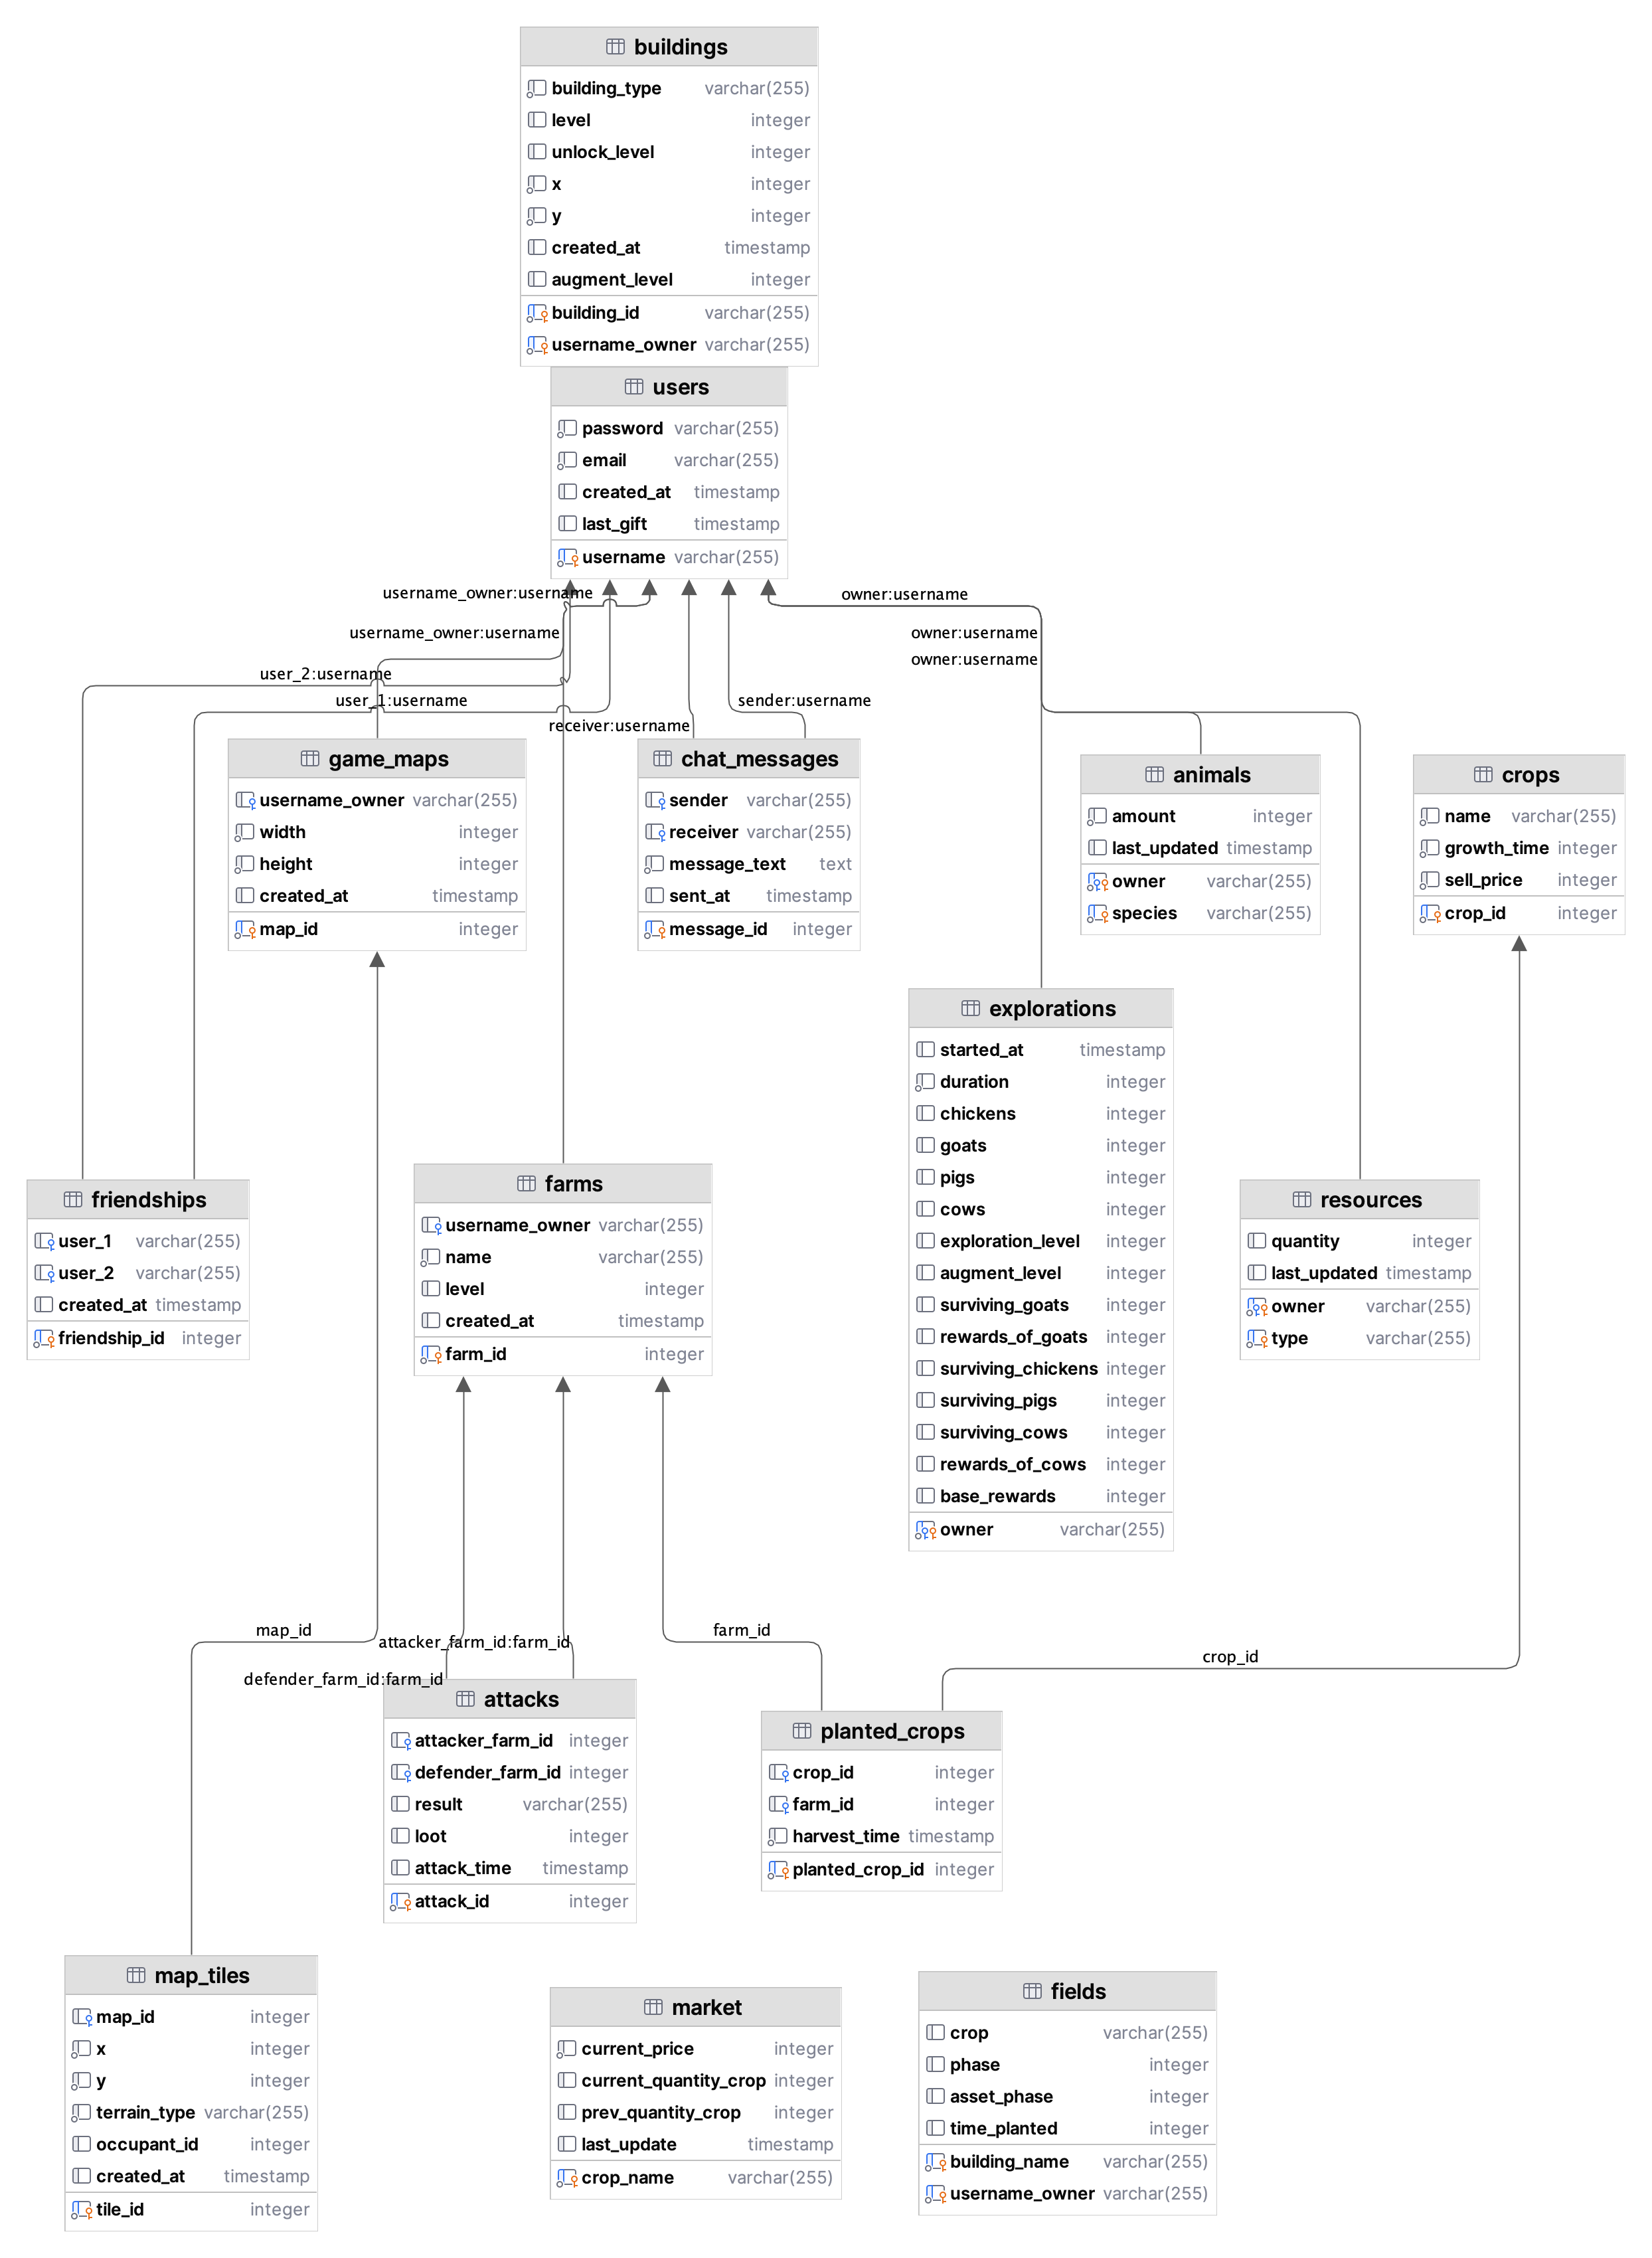
\includegraphics[width=\textwidth]{img/db-diagram.png}
    \caption{Final Database Schema}
    \label{fig:db_schema}
\end{figure}

\subsection{Backend Logic}
The backend handles requests from the client, processes game logic, and interacts with the database. It ensures that all player actions are reflected in real-time and manages the continuous accumulation of resources even when the player is offline.
\subsubsection{Login and Authentication Feature}
\paragraph{Login Feature}
The login functionality is critical for user authentication, allowing users to securely access their accounts.
\begin{itemize}
    \item \textbf{Endpoint} The route `/auth/login`(methods=['GET', 'POST']) handles the login requests.
    \item \textbf{Form Processing} When a POST request is received, the server retrieves the username and password from the form data.
    \item \textbf{User Validation} The user details are fetched from the database using user\_data\_access.get\_user(username). The password is verified using werkzeug\_check\_password\_hash.
    \item \textbf{Session Management}  If the credentials are valid, login\_user(user\_record) is called to log the user in, using Flask-Login to handle the session.
    \item \textbf{Response} After successful login, users are redirected to the game interface or admin panel based on their role
    \item \textbf{Error Handling} If login fails, an error message is displayed.
\end{itemize}
\paragraph{Registration Feature}
Registration allows new users to create accounts by providing their username, password, and email.
\begin{itemize}
    \item \textbf{Endpoint} The route `/auth/register`(methods=['GET', 'POST']) handles the registration requests.
    \item \textbf{User Creation} On receiving a POST request, it attempts to create a new user record with the provided details. The password should ideally be hashed before storage (though hashing is not explicitly mentioned in the provided code).
    \item \textbf{Account initialization} If the user is successfully added to the database, the system initializes the user's game environment, including creating a default map and initializing resources using GameServices.
    \item \textbf{Response} Successful registration redirects the user to the login page. If registration fails (e.g., if the username is already taken), an error message is provided.
\end{itemize}
\paragraph{Logout Feature}
The logout functionality securely ends a user's session.
\begin{itemize}
    \item \textbf{Endpoint} The route `/auth/logout` logs the user out by calling logout\_user() from Flask-Login.
\end{itemize}
\subsubsection{Friends and Messaging Feature}
The friends and messaging features are central to fostering a community environment and enabling social interactions within the game.
\paragraph{Friends Feature:}
The backend supports functionalities related to the management of friendships between users. Users can add new friends, and view their list of friends. The implementation involves:
\begin{itemize}
    \item \textbf{Friend Request Management:} Users add friends using a specific API endpoint that updates the database to include a new friendship. This is implemented in the endpoint defined in \texttt{api.py} (see line 96). The endpoint is:
    \begin{verbatim}
    .../add_friend/<string:friend_name>
    \end{verbatim}
    By utilizing the User Data Access, we retrieve data for both the current user and the prospective friend, converting this information into user objects through the get\_user function. Once we have the user data, we create a new friendship by employing the add\_friendship method from the Friendship Data Access class.
    \item \textbf{List of Friends:} Users can retrieve their list of friends through an API call, which fetches the data from the database and returns it in a formatted JSON array. This feature ensures that users can easily access and interact with their friends list. The relevant API call is implemented in \texttt{views/friends.py} (see line 43). The endpoint is:
    \begin{verbatim}
    .../api/friends
    \end{verbatim}
    \item \textbf{Visit Friends World:} The system allows users to visit their friends' farms, fostering engagement and interaction between players. This feature is implemented in the frontend, where users can navigate to their friends' maps and view their progress.

    The backend enables the user to see the map and buildings of there friends. This is done by fetching the building information of the user that is being visited.
\end{itemize}

\paragraph{Messaging Feature:}
These features not only enhance user engagement but also contribute to the game's social dynamics, making the gaming experience more interactive and enjoyable for users.
\begin{itemize}
    \item \textbf{Messaging window:} You can retrieve the previous messages from the right friend. this is done by using  A GET request that is made to the API endpoint, where friend-name is the name of the friend whose messages are being fetched.
    \begin{verbatim}
    /api/messages/${friend_name}
    \end{verbatim}
    \item \textbf{Message Element Creation:} A div element is created for the message, with a class of received if the message is from the friend, or sent if it is from the current user. The message content is added to this div.
    \item \textbf{Timestamp Divider:}  If there is an hour or more difference between the current message and the last message, a timestamp divider is added to indicate the time.
\end{itemize}




\subsubsection{Leaderboard Feature}
The backend manages the leaderboard by fetching and calculating user scores, sorting them, and handling specific leaderboard queries. Here's how it is structured:
\begin{itemize}
    \item \textbf{Fetch and Calculate Scores:} The route \begin{verbatim}`@api/leaderboard`\end{verbatim} is used for handling GET requests for the leaderboard. It retrieves all users from the database via user\_data\_access.get\_all\_users(). For each user, it calculates the total score by summing up the resources associated with each user, fetched by resource\_data\_access.get\_resources(user.username).
    \item \textbf{Sort and Rank Users:} Users are sorted by their calculated scores in descending order. The backend extracts the top three users to represent the leading positions on the leaderboard. Additionally, it retrieves two friends of the current user to include in the leaderboard for more personalized competition.
    \item \textbf{Ensure Inclusion of Current User:} The system checks if the current user is among the top users or friends listed. If not, the current user is also added to the leaderboard. It then removes duplicates and finalizes a ranked list of unique users.
    \item \textbf{Return Leaderboard Data:} The backend returns the leaderboard data in JSON format, including the user's rank, username, and score. This data is then displayed on the frontend for users to view and engage with.
\end{itemize}

\subsubsection{Market Feature}
The backend manages the market by storing the current price and adjusting it based on user sales of a given crop. This process occurs in intervals of 1 minute using past and current sales data:
route : \begin{verbatim}`@api/update-market`\end{verbatim}
\begin{itemize}
    \item \textbf{update price:} Calculates a new price for a crop. Adjusts the price based on the current count and a random factor. Constrains the new price within a specific range. Returns the calculated new price.
    \item \textbf{update market:} Handles POST requests for updating market data. Retrieves current market data for a specific crop. If 1 minute has passed since the last update, calculates and updates the price using the update\_price function. Updates the market data with the current sales and price. Creates a new entry with a default price if no existing market data is found. Returns a response indicating the success or failure of the update.
    \item \textbf{fetch price:} Handles GET requests to fetch the current price of a crop. Retrieves market data for the requested crop. Updates the price using the update\_price function if needed. Returns the current price of the crop in the response.
\end{itemize}

\subsubsection{Building Feature}
The backend manages the buildings by storing, updating or fatching the requested building\_data:
route : \begin{verbatim}`@api/building-map`\end{verbatim}
\begin{itemize}
    \item \textbf{update\_map Function:} inserts a given building json in the database. If it exists, it updates, else it creates a new entry.
    \item \textbf{fetch\_building\_information Route:} Handles GET requests to the requested building info. if the requested building does not exist, returns an error.
\end{itemize}


\subsection{Frontend Interface}
The frontend provides an interactive and user-friendly interface using React, allowing players to engage with the game seamlessly. It features a map view for navigating different parts of the farm and a market interface for selling produce.
\subsubsection{Login and Authentication Feature}
\paragraph{Login Page}
The login page offers a straightforward interface for existing users to access their accounts.
\begin{itemize}
    \item \textbf{HTML and CSS:} Structure: The login form is embedded within a div element styled with a form-container class. It includes input fields for username and password. Styling: Stylesheets for authentication (auth.css) and footer (footer.css) are linked to maintain consistency in appearance with the rest of the application. The Press Start 2P font from Google Fonts enhances the retro aesthetic of the app.
    \item \textbf{JavaScript:} Dynamic Visual Feedback: JavaScript is used to provide visual feedback on the login button. It changes the button's image when pressed and released, helping confirm user interaction. Form Submission: The form posts data to the /auth/login endpoint, handling user authentication in the backend.
\end{itemize}
\paragraph{Registration Page}
The registration page allows new users to create an account by providing essential information such as username, password, and email.
\begin{itemize}
    \item \textbf{HTML and CSS:} Extended Form: Similar to the login form but includes an additional field for email to accommodate the registration process. Consistent Styling: Utilizes the same CSS files as the login page for a uniform look and feel.
    \item \textbf{JavaScript:} Button Feedback: Implements the same interactive feedback for the registration button, enhancing user experience during the account creation process.
\end{itemize}

\subsubsection{MAIN GAME WORLD}
The \textit{main game world} consists of several HTML canvases layered on top of each other, each with their own unique
JavaScript classes to provide the right functionality. These canvases display 16x16 tiles scaled to a variable size and
fill the entire screen. The player can click and drag the screen to look around the game world, interact with buildings,
and use the appropriate UI to navigate different parts of the game.

After logging in, the player gets redirected to \texttt{https://"baseLink"/game/} which fetches \texttt{game.html}. This
file is the most important HTML, as it connects and fetches every other file. It includes the UI HTML, the pop-up HTML,
sets and positions the canvases, and links \texttt{canvas.js}. All the canvases have their own set of tiles which are
pre-fetched and stored during the initialization period. This is needed for instantaneous loading; otherwise, a fetch
delay is noticeable during runtime.

The HTML UI elements sit on top of these canvases and utilize CSS styling. The only technologies used are JavaScript,
HTML, and CSS.


\paragraph{canvas.js} This file is most important for initializing the game. It creates all the JavaScript classes used
throughout the main game in the correct order (some classes depend on other classes). It is also responsible for
correctly resizing all the layered canvases when the browser window's size is changed by the user. Additionally the
initialize() functions of some classes are called. These async functions perform all the correct fetches for the
asset's. Then the resize event gets linked and the ticker class gets started.

\paragraph{Terrain Layer}
The terrain layer provides functionality for correctly displaying the terrain tiles and is the lowest layered canvas,
providing as a sort of background layer.
The map is procedurally generated with a map size with width 58 and height 43
with the usable part of the map being the middle 50x35 as 4 tiles are used as border/padding around the map. This padding
consists of 3 water tiles and a grass water border. As for the map itself it is generated using a generate\_water\_positions()
function which takes parameters the actual width (50) and height (35), number of lakes (default = 8), minimum lake size
(default = 3 tiles) and the maximum lake size (default = 10 tiles) and returns the positions where water should be generated.
The actual variation of the tile is then randomly chosen out of a set of assets. There are default assets and special assets
which contain special things (stone, logs, bushes etc.).
The map is stored as a 2D array of strings that refer to their tile png name.
All these assets were fetched beforehand and stored in a map with the tile name as the key. The 'drawTiles()' function
uses the map array together with the camera location to correctly draw the tiles on the screen. This function gets
called many times throughout the code every time there's an adjustment and the tiles need to be redrawn. When dragging
the screen the appropriate move functions of the map get called which change the camera location and redraw the screen.

After starting the game you may notice some tiles are being animated. This is accomplished by utilizing the tick()
function and going through the terrain map array, changing specific tiles to the consequent tile in the animation and
redrawing them.

\paragraph{Building Layer} The building layer works similarly to the terrain layer in terms of rendering the tiles but
there are some distinctions and  additional features. The way the building map is saved differs from the the terrain
layer. The buildings and building information are saved in a json structure. (opslag methode moet ge\"update worden dus
hier is nog geen documentatie voor).

The building layer provides support for interacting with buildings. To move a building you can click (without dragging),
after which the building is locked to the mouse. Move the mouse, then click again to place the building. When attempting
to place a building on an invalid location the building simply doesn't get placed and stays attached to the mouse.
Invalid locations include other buildings and water tiles. When trying to drag a building outside the window or outside
the map bounds the building doesn't move any further in a way such that it is never in an impossible location. You can
drag the screen while moving a building to easily move around the map without needing to let go of the building.

When moving a building it gets rendered on top of all other buildings to avoid it from going underneath other structures
around the map. This would lead to a somewhat strange visual otherwise.

\paragraph{Building Pop-up} When right-clicking on a building, a HTML pop-up shows up on the right side of the screen.
This is used to display various details about the building of interest and also allows you to upgrade the building. The
pop-up contains a "Building Info" title, the name of the type of building, a small text with some information (namely
the purpose of the building). On top of that there are, depending on the type of building, potentially some stats that
include the level the building is at and other stats like upgrade cost, defense, eggs/hour, etc. Lastly there is an
upgrade button, a close button and augment button that are all animated when clicked.

When right-clicking another building while a pop-up is already open, a switch animation is displayed to make clear that
you are switching to the information of a different building. When right-clicking the same building twice this animation
doesn't happen. Lastly when doing almost any other action like dragging the screen and moving a building the pop-up
automatically closes.

\paragraph{Main UI} The header and footer HTML provide the user with buttons for easy access to different parts of the
game as well as displaying some useful information such as the amount of coins and produce the player has.

\paragraph{Ticker class} This JavaScript code utilizes the observer pattern. During initialization, classes can
subscribe to this class, then when the  ticker starts it will call the tick() function on every subscribed class every
set milliseconds (1000/24 ms to get 24 frames/second). Classes can then use this function to implement timing sensitive
functionality, namely animations.

\paragraph{User Input Handler} This is a class that has set up all the event listeners needed to detect useful user
input in its constructor. Like the Ticker class it also uses an observer pattern approach, where all classes that
potentially need to know about user input get added in the initialization phase of the game.

In this project a click on any of the canvases only gets registered on the mouse up event. This is because we clearly
want to differentiate between a click and a drag. To achieve this the user input handler stores the mouse down location.
On the mouse up event it compares the current location to the mouse down location and when this distance is smaller then
5 pixels in the x and y direction, a click is registered. This margin ensures that when the user accidentally moves the
mouse a few pixels, the input still gets registered as a click.

In order to check on what canvas the user intended to click, a trickle-down method is used. The input handler first
checks the first class in the list and calls the 'handleClickInput(x,y)' function on this class. This function will then
return a boolean whether the click was applicable to the class or not. If not, the handleClick function is called on the
next layer's class and so on.


\subsubsection{Friends and Messaging Feature}
The friends and messaging features are central to fostering a community environment and enabling social interactions within the game.
\paragraph{Friends Feature}
\begin{itemize}
    \item \textbf{HTML and CSS:} The friends/dashboard.html file structures the friends page, displaying the user's friends list. The friends.css file styles the page, ensuring a consistent design with the rest of the application.
    \item \textbf{JavaScript:} The loadFriends() function fetches the user's friends list from the backend API. It populates the friends table in the HTML dynamically, ensuring that users can easily view and interact with their friends. Error handling is included to manage and alert users in case of API failures. The visitFriendsWorld() function allows users to visit their friends' farms, enhancing social interactions within the game.
\end{itemize}

\paragraph{Mesaging Feature}
\begin{itemize}
    \item \textbf{HTML and CSS:} The chat-window.html files structures the message window page, displaying a chat window with messages between you and a friend. The chat-window.html section css file styles the page, ensuring a consistent design with the rest of the application.
    \item \textbf{JavaScript:}The loadChat() function handles loading the chat messages for a specific friend. Updates the chat window title to the friend's name, also let you as user visit your friends world with the visit world button. The chat messages  are fetched from the server, processes them, and displays them in the chat window.
\end{itemize}

\subsubsection{Leaderboard Feature}
\begin{itemize}
    \item \textbf{HTML and CSS:} The leaderboard.html contains the HTML structure, including a table where the leaderboard will be dynamically populated. The CSS file leaderboard.css styles the leaderboard page, ensuring a visually appealing and consistent design.
    \item \textbf{JavaScript:} A JavaScript function loadLeaderboard() (event handling; this function is triggered when document content is fully loaded) is responsible for fetching the leaderboard data from the backend API. Upon successful fetch, it populates the leaderboard table in the HTML dynamically. Error handling is incorporated to manage and alert users in case of failures in data retrieval.
\end{itemize}

\subsubsection{Books}
\begin{itemize}
    \item \textbf{HTML and CSS:} The bookChat.html and bookMarket.html contain the HTML structure of the books, covers and pages (front and back), along with the content for the chat and the market respectively.
    \item \textbf{JavaScript:} There is a JavaScript function: openBook() to open the cover of the book and a closeBook() to close the cover of the book. In addition, you have the goNextPage() function to go to the next page and the goPrevPage() function to go to the previous page. In addition to these functions, there are querySelectors for the covers, pages and buttons
\end{itemize}

\subsubsection{Settings and Sound Feature}
The settings and sound features are integral to creating an immersive and personalized gaming experience, enhancing user engagement and enjoyment within the game.
\paragraph{Settings Feature}
\begin{itemize}
    \item \textbf{HTML and CSS:} The settings.html contains the HTML structure of the settings. This html file creates the buttons needed in the settins: LOG-OUT, SOUND, ZOOM.  The CSS file settings.css styles settings page, matching the design of other pages.
    \item \textbf{JavaScript:} There is a JavaScript file, where the setting functions are implemented. There is a function soundUp() that lets you volume up the sound. The variable countSound keeps this value and stores it in a storage. The value is also given as a parameter to the sound function setVolume(). The same with soundDown(). zoomUpPrecent() is a function that controls the variable tilesize in the the file canvas.js for updating the window size. also with zoomDownPrecent().
\end{itemize}

\paragraph{Sound Feature}
\begin{itemize}
    \item \textbf{HTML and CSS:} The settings.html contains the sound buttons created for this feature.
    \item \textbf{JavaScript:} There is a javascript file sound.js with a class GameSoundManager that contains functions to control the music in the game controlled by the buttons in settings.js.The function setBackgroundMusic() initializes the music being given and plays it when the background button is on in settings. The function setVolume() is given the variable countSound as parameter from the file settings.js and is used to set the right volume for the background music.
\end{itemize}


\section{Challenges and Solutions}
Throughout the development, the team encountered and overcame numerous challenges, such as optimizing database queries and ensuring smooth synchronous player interactions. Specific issues included managing the real-time update of resource levels and implementing secure authentication mechanisms.

\section{Results and Testing}
The game was rigorously tested to ensure functionality across different systems and scenarios. Our testing approach was comprehensive, incorporating automated unit tests, integration tests, and user acceptance testing to cover both the backend and frontend components of our application.
\subsection{Backend Testing}
For backend testing, we utilized Pytest, a powerful and flexible testing tool. Our tests included:
\begin{itemize}
    \item \textbf{Database Connection Tests:} Using \texttt{test\_dbconnection.py}, we verified the stability and reliability of our database connections, ensuring that all interactions with the database handled data correctly and maintained integrity under various conditions.
    \item \textbf{API Functionality Tests:} We conducted extensive testing on our RESTful API endpoints to ensure accurate response statuses and proper data formatting. This included testing:
        \begin{itemize}
            \item \textbf{User Endpoint:} Verified that only administrators could retrieve user data, and that the data was correctly formatted as JSON.
            \item \textbf{Maps Endpoint:} Ensured that map data could only be accessed by administrators, testing for correct map attributes and response format.
            \item \textbf{Resources Endpoint:} Checked both general and specific resource retrieval endpoints for proper authorization checks and JSON formatting.
            \item \textbf{Terrain Map Endpoint:} Tested user-specific access to terrain maps, ensuring the integrity and format of the terrain data returned.
            \item \textbf{Market Data Access:} We insert and fetch new crop elements , to check if the database requests work.
            \item \textbf{Building Data Access:} We check if the database is updated correctly when inserting new elements and fetching them.
            \item \textbf{Friendships Endpoint:} Assured that users could reliably retrieve their list of friends, with responses properly formatted as JSON arrays.
            \item \textbf{Chat Endpoint:} Confirmed functionality for retrieving chat messages between users, focusing on correct data handling and security measures.
        \end{itemize}
    These tests not only verified proper access control and data integrity but also ensured that our server effectively handled errors and returned appropriate status codes under various scenarios.
    \item \textbf{Data Access Layer Tests:}
    \begin{itemize}
        \item \textbf{User Data Access:} Using \texttt{test\_user\_data\_access.py}, we tested CRUD operations for user data to ensure accurate storage, retrieval, updating, and deletion of user information.
        \item \textbf{Map Data Access:} In \texttt{test\_map\_data\_access.py}, we verified the functionality of our map management system, ensuring that map data manipulations were handled correctly.
        \item \textbf{Tile Data Access:} The \texttt{test\_tile\_data\_access.py} allowed us to ensure that tile-based operations, crucial for the game's map functionality, were accurate and efficient.
        \item \textbf{Resource Data Access:} Through \texttt{test\_resource\_data\_access.py}, we tested the handling of game resources, confirming the correct implementation of resource accumulation and usage.
        \item \textbf{Friendship Data Access:} With \texttt{test\_friendship\_data\_access.py}, we assessed the systems managing player interactions and relationships within the game.
        \item \textbf{Chat Message Data Access:} Using \texttt{test\_chatmessage\_data\_access.py}, we evaluated the functionality of in-game chat systems, ensuring reliable and secure message delivery and storage.
        \item \textbf{Building Data Access:} Using \texttt{test\_building\_data\_access.py}, we ensure correct retrieval of building information
        \item \textbf{Market Data Access:} Using \texttt{test\_market\_data\_access.py}, we check if the sale count if updated correctly using the database
    \end{itemize}
    \item \textbf{Integration Tests:} We conducted extensive tests to ensure that these individual components functioned together seamlessly, simulating real-world usage to detect any integration issues.
\end{itemize}
These targeted tests helped us to systematically validate each aspect of our backend, ensuring robustness and reliability throughout the game's infrastructure.

\subsection{Frontend Testing}
Frontend testing was conducted using a combination of Jasmine and manual testing, focusing on the interactive aspects of our application:
\begin{itemize}
    \item \textbf{UI Component Tests:} We tested the rendering and behavior of graphical components, such as the game map and resource widgets, to ensure they behaved consistently across different browsers and resolutions.
    \item \textbf{User Interaction Tests:} We simulated user interactions such as clicking, dragging, clicking button and resizing the browser window to ensure the UI responded correctly and efficiently without errors or unexpected behavior.
\end{itemize}
\subsection{User Acceptance Testing}
User acceptance testing was carried out with a group of target users who provided valuable feedback on the usability and overall experience of the game. This feedback was crucial in refining the gameplay mechanics and interface, leading to several iterations that enhanced user engagement and satisfaction.
\subsection{Continuous Integration}
We integrated continuous integration tools into our development process, allowing us to automatically run tests upon every commit to our version control system. This helped us quickly identify and rectify issues early in the development cycle, improving product quality and reducing time to deployment.
Overall, our structured and thorough approach to testing ensured that 'FarmClash' was robust, user-friendly, and scalable, ready to handle the demands of real-world usage by players across the globe.

\section{User Manual}
\subsection{Installation}
Details the steps required to install and run the game locally, as outlined in the README document.

\subsection{Gameplay}
Explains basic gameplay mechanics, how to interact within the game, and strategies for new players. It covers logging in, starting a farm, upgrading buildings, and interacting with other players.

\section{Conclusion}
The project successfully demonstrates the application of database and web development skills in creating a functional and engaging multiplayer game. Future enhancements could include more complex defense strategies and a broader range of market dynamics.

\section{References}
List all references and resources used during the development of the project.

\end{document}
